
%% bare_conf.tex
%% V1.3
%% 2007/01/11
%% by Michael Shell
%% See:
%% http://www.michaelshell.org/
%% for current contact information.
%%
%% This is a skeleton file demonstrating the use of IEEEtran.cls
%% (requires IEEEtran.cls version 1.7 or later) with an IEEE conference paper.
%%
%% Support sites:
%% http://www.michaelshell.org/tex/ieeetran/
%% http://www.ctan.org/tex-archive/macros/latex/contrib/IEEEtran/
%% and
%% http://www.ieee.org/

%%*************************************************************************
%% Legal Notice:
%% This code is offered as-is without any warranty either expressed or
%% implied; without even the implied warranty of MERCHANTABILITY or
%% FITNESS FOR A PARTICULAR PURPOSE! 
%% User assumes all risk.
%% In no event shall IEEE or any contributor to this code be liable for
%% any damages or losses, including, but not limited to, incidental,
%% consequential, or any other damages, resulting from the use or misuse
%% of any information contained here.
%%
%% All comments are the opinions of their respective authors and are not
%% necessarily endorsed by the IEEE.
%%
%% This work is distributed under the LaTeX Project Public License (LPPL)
%% ( http://www.latex-project.org/ ) version 1.3, and may be freely used,
%% distributed and modified. A copy of the LPPL, version 1.3, is included
%% in the base LaTeX documentation of all distributions of LaTeX released
%% 2003/12/01 or later.
%% Retain all contribution notices and credits.
%% ** Modified files should be clearly indicated as such, including  **
%% ** renaming them and changing author support contact information. **
%%
%% File list of work: IEEEtran.cls, IEEEtran_HOWTO.pdf, bare_adv.tex,
%%                    bare_conf.tex, bare_jrnl.tex, bare_jrnl_compsoc.tex
%%*************************************************************************

% *** Authors should verify (and, if needed, correct) their LaTeX system  ***
% *** with the testflow diagnostic prior to trusting their LaTeX platform ***
% *** with production work. IEEE's font choices can trigger bugs that do  ***
% *** not appear when using other class files.                            ***
% The testflow support page is at:
% http://www.michaelshell.org/tex/testflow/



% Note that the a4paper option is mainly intended so that authors in
% countries using A4 can easily print to A4 and see how their papers will
% look in print - the typesetting of the document will not typically be
% affected with changes in paper size (but the bottom and side margins will).
% Use the testflow package mentioned above to verify correct handling of
% both paper sizes by the user's LaTeX system.
%
% Also note that the "draftcls" or "draftclsnofoot", not "draft", option
% should be used if it is desired that the figures are to be displayed in
% draft mode.
%
\documentclass[conference]{IEEEtran}
% Add the compsoc option for Computer Society conferences.
%
% If IEEEtran.cls has not been installed into the LaTeX system files,
% manually specify the path to it like:
% \documentclass[conference]{../sty/IEEEtran}





% Some very useful LaTeX packages include:
% (uncomment the ones you want to load)


% *** MISC UTILITY PACKAGES ***
%
%\usepackage{ifpdf}
% Heiko Oberdiek's ifpdf.sty is very useful if you need conditional
% compilation based on whether the output is pdf or dvi.
% usage:
% \ifpdf
%   % pdf code
% \else
%   % dvi code
% \fi
% The latest version of ifpdf.sty can be obtained from:
% http://www.ctan.org/tex-archive/macros/latex/contrib/oberdiek/
% Also, note that IEEEtran.cls V1.7 and later provides a builtin
% \ifCLASSINFOpdf conditional that works the same way.
% When switching from latex to pdflatex and vice-versa, the compiler may
% have to be run twice to clear warning/error messages.






% *** CITATION PACKAGES ***
%
%\usepackage{cite}
% cite.sty was written by Donald Arseneau
% V1.6 and later of IEEEtran pre-defines the format of the cite.sty package
% \cite{} output to follow that of IEEE. Loading the cite package will
% result in citation numbers being automatically sorted and properly
% "compressed/ranged". e.g., [1], [9], [2], [7], [5], [6] without using
% cite.sty will become [1], [2], [5]--[7], [9] using cite.sty. cite.sty's
% \cite will automatically add leading space, if needed. Use cite.sty's
% noadjust option (cite.sty V3.8 and later) if you want to turn this off.
% cite.sty is already installed on most LaTeX systems. Be sure and use
% version 4.0 (2003-05-27) and later if using hyperref.sty. cite.sty does
% not currently provide for hyperlinked citations.
% The latest version can be obtained at:
% http://www.ctan.org/tex-archive/macros/latex/contrib/cite/
% The documentation is contained in the cite.sty file itself.






% *** GRAPHICS RELATED PACKAGES ***
%
\ifCLASSINFOpdf
  \usepackage[pdftex]{graphicx}
  % declare the path(s) where your graphic files are
  % \graphicspath{{../pdf/}{../jpeg/}}
  % and their extensions so you won't have to specify these with
  % every instance of \includegraphics
  % \DeclareGraphicsExtensions{.pdf,.jpeg,.png}
\else
  % or other class option (dvipsone, dvipdf, if not using dvips). graphicx
  % will default to the driver specified in the system graphics.cfg if no
  % driver is specified.
  % \usepackage[dvips]{graphicx}
  % declare the path(s) where your graphic files are
  % \graphicspath{{../eps/}}
  % and their extensions so you won't have to specify these with
  % every instance of \includegraphics
  % \DeclareGraphicsExtensions{.eps}
\fi
% graphicx was written by David Carlisle and Sebastian Rahtz. It is
% required if you want graphics, photos, etc. graphicx.sty is already
% installed on most LaTeX systems. The latest version and documentation can
% be obtained at: 
% http://www.ctan.org/tex-archive/macros/latex/required/graphics/
% Another good source of documentation is "Using Imported Graphics in
% LaTeX2e" by Keith Reckdahl which can be found as epslatex.ps or
% epslatex.pdf at: http://www.ctan.org/tex-archive/info/
%
% latex, and pdflatex in dvi mode, support graphics in encapsulated
% postscript (.eps) format. pdflatex in pdf mode supports graphics
% in .pdf, .jpeg, .png and .mps (metapost) formats. Users should ensure
% that all non-photo figures use a vector format (.eps, .pdf, .mps) and
% not a bitmapped formats (.jpeg, .png). IEEE frowns on bitmapped formats
% which can result in "jaggedy"/blurry rendering of lines and letters as
% well as large increases in file sizes.
%
% You can find documentation about the pdfTeX application at:
% http://www.tug.org/applications/pdftex





% *** MATH PACKAGES ***
%
%\usepackage[cmex10]{amsmath}
% A popular package from the American Mathematical Society that provides
% many useful and powerful commands for dealing with mathematics. If using
% it, be sure to load this package with the cmex10 option to ensure that
% only type 1 fonts will utilized at all point sizes. Without this option,
% it is possible that some math symbols, particularly those within
% footnotes, will be rendered in bitmap form which will result in a
% document that can not be IEEE Xplore compliant!
%
% Also, note that the amsmath package sets \interdisplaylinepenalty to 10000
% thus preventing page breaks from occurring within multiline equations. Use:
%\interdisplaylinepenalty=2500
% after loading amsmath to restore such page breaks as IEEEtran.cls normally
% does. amsmath.sty is already installed on most LaTeX systems. The latest
% version and documentation can be obtained at:
% http://www.ctan.org/tex-archive/macros/latex/required/amslatex/math/





% *** SPECIALIZED LIST PACKAGES ***
%
%\usepackage{algorithmic}
% algorithmic.sty was written by Peter Williams and Rogerio Brito.
% This package provides an algorithmic environment fo describing algorithms.
% You can use the algorithmic environment in-text or within a figure
% environment to provide for a floating algorithm. Do NOT use the algorithm
% floating environment provided by algorithm.sty (by the same authors) or
% algorithm2e.sty (by Christophe Fiorio) as IEEE does not use dedicated
% algorithm float types and packages that provide these will not provide
% correct IEEE style captions. The latest version and documentation of
% algorithmic.sty can be obtained at:
% http://www.ctan.org/tex-archive/macros/latex/contrib/algorithms/
% There is also a support site at:
% http://algorithms.berlios.de/index.html
% Also of interest may be the (relatively newer and more customizable)
% algorithmicx.sty package by Szasz Janos:
% http://www.ctan.org/tex-archive/macros/latex/contrib/algorithmicx/




% *** ALIGNMENT PACKAGES ***
%
%\usepackage{array}
% Frank Mittelbach's and David Carlisle's array.sty patches and improves
% the standard LaTeX2e array and tabular environments to provide better
% appearance and additional user controls. As the default LaTeX2e table
% generation code is lacking to the point of almost being broken with
% respect to the quality of the end results, all users are strongly
% advised to use an enhanced (at the very least that provided by array.sty)
% set of table tools. array.sty is already installed on most systems. The
% latest version and documentation can be obtained at:
% http://www.ctan.org/tex-archive/macros/latex/required/tools/


%\usepackage{mdwmath}
%\usepackage{mdwtab}
% Also highly recommended is Mark Wooding's extremely powerful MDW tools,
% especially mdwmath.sty and mdwtab.sty which are used to format equations
% and tables, respectively. The MDWtools set is already installed on most
% LaTeX systems. The lastest version and documentation is available at:
% http://www.ctan.org/tex-archive/macros/latex/contrib/mdwtools/


% IEEEtran contains the IEEEeqnarray family of commands that can be used to
% generate multiline equations as well as matrices, tables, etc., of high
% quality.


%\usepackage{eqparbox}
% Also of notable interest is Scott Pakin's eqparbox package for creating
% (automatically sized) equal width boxes - aka "natural width parboxes".
% Available at:
% http://www.ctan.org/tex-archive/macros/latex/contrib/eqparbox/





% *** SUBFIGURE PACKAGES ***
%\usepackage[tight,footnotesize]{subfigure}
% subfigure.sty was written by Steven Douglas Cochran. This package makes it
% easy to put subfigures in your figures. e.g., "Figure 1a and 1b". For IEEE
% work, it is a good idea to load it with the tight package option to reduce
% the amount of white space around the subfigures. subfigure.sty is already
% installed on most LaTeX systems. The latest version and documentation can
% be obtained at:
% http://www.ctan.org/tex-archive/obsolete/macros/latex/contrib/subfigure/
% subfigure.sty has been superceeded by subfig.sty.



%\usepackage[caption=false]{caption}
%\usepackage[font=footnotesize]{subfig}
% subfig.sty, also written by Steven Douglas Cochran, is the modern
% replacement for subfigure.sty. However, subfig.sty requires and
% automatically loads Axel Sommerfeldt's caption.sty which will override
% IEEEtran.cls handling of captions and this will result in nonIEEE style
% figure/table captions. To prevent this problem, be sure and preload
% caption.sty with its "caption=false" package option. This is will preserve
% IEEEtran.cls handing of captions. Version 1.3 (2005/06/28) and later 
% (recommended due to many improvements over 1.2) of subfig.sty supports
% the caption=false option directly:
%\usepackage[caption=false,font=footnotesize]{subfig}
%
% The latest version and documentation can be obtained at:
% http://www.ctan.org/tex-archive/macros/latex/contrib/subfig/
% The latest version and documentation of caption.sty can be obtained at:
% http://www.ctan.org/tex-archive/macros/latex/contrib/caption/




% *** FLOAT PACKAGES ***
%
%\usepackage{fixltx2e}
% fixltx2e, the successor to the earlier fix2col.sty, was written by
% Frank Mittelbach and David Carlisle. This package corrects a few problems
% in the LaTeX2e kernel, the most notable of which is that in current
% LaTeX2e releases, the ordering of single and double column floats is not
% guaranteed to be preserved. Thus, an unpatched LaTeX2e can allow a
% single column figure to be placed prior to an earlier double column
% figure. The latest version and documentation can be found at:
% http://www.ctan.org/tex-archive/macros/latex/base/



%\usepackage{stfloats}
% stfloats.sty was written by Sigitas Tolusis. This package gives LaTeX2e
% the ability to do double column floats at the bottom of the page as well
% as the top. (e.g., "\begin{figure*}[!b]" is not normally possible in
% LaTeX2e). It also provides a command:
%\fnbelowfloat
% to enable the placement of footnotes below bottom floats (the standard
% LaTeX2e kernel puts them above bottom floats). This is an invasive package
% which rewrites many portions of the LaTeX2e float routines. It may not work
% with other packages that modify the LaTeX2e float routines. The latest
% version and documentation can be obtained at:
% http://www.ctan.org/tex-archive/macros/latex/contrib/sttools/
% Documentation is contained in the stfloats.sty comments as well as in the
% presfull.pdf file. Do not use the stfloats baselinefloat ability as IEEE
% does not allow \baselineskip to stretch. Authors submitting work to the
% IEEE should note that IEEE rarely uses double column equations and
% that authors should try to avoid such use. Do not be tempted to use the
% cuted.sty or midfloat.sty packages (also by Sigitas Tolusis) as IEEE does
% not format its papers in such ways.





% *** PDF, URL AND HYPERLINK PACKAGES ***
%
\usepackage{url}
\usepackage{listings}
% url.sty was written by Donald Arseneau. It provides better support for
% handling and breaking URLs. url.sty is already installed on most LaTeX
% systems. The latest version can be obtained at:
% http://www.ctan.org/tex-archive/macros/latex/contrib/misc/
% Read the url.sty source comments for usage information. Basically,
% \url{my_url_here}.





% *** Do not adjust lengths that control margins, column widths, etc. ***
% *** Do not use packages that alter fonts (such as pslatex).         ***
% There should be no need to do such things with IEEEtran.cls V1.6 and later.
% (Unless specifically asked to do so by the journal or conference you plan
% to submit to, of course. )


% correct bad hyphenation here
\hyphenation{op-tical net-works semi-conduc-tor}


\begin{document}
%
% paper title
% can use linebreaks \\ within to get better formatting as desired
\title{File-System Traces Analysis}


% author names and affiliations
% use a multiple column layout for up to three different
% affiliations
\author{\IEEEauthorblockN{Sudhir Kasanavesi}
\IEEEauthorblockA{Department of Computer Science\\
Stony Brook University\\
SBU ID: 108492541}
\and
\IEEEauthorblockN{Nihar Konireddy}
\IEEEauthorblockA{Department of Computer Science\\
Stony Brook University\\
SBU ID: 108395318}
\and
\IEEEauthorblockN{Kalyan Chandra Chintalapati}
\IEEEauthorblockA{Department of Computer Science\\
Stony Brook University\\
SBU ID: 108080090}}

% conference papers do not typically use \thanks and this command
% is locked out in conference mode. If really needed, such as for
% the acknowledgment of grants, issue a \IEEEoverridecommandlockouts
% after \documentclass

% for over three affiliations, or if they all won't fit within the width
% of the page, use this alternative format:
% 
%\author{\IEEEauthorblockN{Michael Shell\IEEEauthorrefmark{1},
%Homer Simpson\IEEEauthorrefmark{2},
%James Kirk\IEEEauthorrefmark{3}, 
%Montgomery Scott\IEEEauthorrefmark{3} and
%Eldon Tyrell\IEEEauthorrefmark{4}}
%\IEEEauthorblockA{\IEEEauthorrefmark{1}School of Electrical and Computer Engineering\\
%Georgia Institute of Technology,
%Atlanta, Georgia 30332--0250\\ Email: see http://www.michaelshell.org/contact.html}
%\IEEEauthorblockA{\IEEEauthorrefmark{2}Twentieth Century Fox, Springfield, USA\\
%Email: homer@thesimpsons.com}
%\IEEEauthorblockA{\IEEEauthorrefmark{3}Starfleet Academy, San Francisco, California 96678-2391\\
%Telephone: (800) 555--1212, Fax: (888) 555--1212}
%\IEEEauthorblockA{\IEEEauthorrefmark{4}Tyrell Inc., 123 Replicant Street, Los Angeles, California 90210--4321}}




% use for special paper notices
%\IEEEspecialpapernotice{(Invited Paper)}




% make the title area
\maketitle


\section{abstract}
%\boldmath
\indent
Traces are good sources of information in understanding the workload 
characteristics of a system [1]. A good trace analysis helps in understanding 
the behavior of the system under a real-time workload and these results would 
help in optimization of the system resources. File-system traces, in particular 
have been used for file system evaluation, user behavior analysis, file-system 
debugging and intrusion detection [3]. But traces tend to be large, hard to use 
and share. Often, however, researchers are not interested in the precise details
stored in a bulky trace, but rather in some statistical properties found in the 
traces - properties that affect their system's behavior under load [1].\\
\indent
Network File System (NFS) is by far the most widely used file-system today. 
NFS client sends requests using Remote Procedure Call (RPC) to the server. 
NFS Server translates these RPC requests and accesses the local physical file system. 
NFS traces can be captured by sniffing the ethernet packets since the request-reply 
between client and server is achieved using RPC. The packets which are captured 
consists of NFS calls and replys, they have to be decoded and then recorded in the 
trace. \\
\indent
This paper aims at providing a framework to analyze the network file 
system. We have built a system that extracts some of the desired properties required 
for analyzing Network File System (NFS) Version3 and convert it
 to the DataSeries[2] format. This is fed to the analyzer built as a part of the system 
for analyzing several workloads. It does some basic analysis such as determining the number of
NFS v3 procedures on a given workload, find the READ and WRITE I/O sizes etc on the traces captured. The network traffic is captured by tshark, network protocol 
analyzer. The results of our analyzer are evaluated with the "dsstatgroupby" tool which is a part of DataSeries [2] tools. Our system currently extracts few desirable properties from a subset of NFS V3 
procedures and can be extended to make the user specify the properties which they intend to analyze.\\

% IEEEtran.cls defaults to using nonbold math in the Abstract.
% This preserves the distinction between vectors and scalars. However,
% if the conference you are submitting to favors bold math in the abstract,
% then you can use LaTeX's standard command \boldmath at the very start
% of the abstract to achieve this. Many IEEE journals/conferences frown on
% math in the abstract anyway.

% no keywords




% For peer review papers, you can put extra information on the cover
% page as needed:
% \ifCLASSOPTIONpeerreview
% \begin{center} \bfseries EDICS Category: 3-BBND \end{center}
% \fi
%
% For peerreview papers, this IEEEtran command inserts a page break and
% creates the second title. It will be ignored for other modes.
\IEEEpeerreviewmaketitle



\section{Introduction}
File system trace analysis would give a comprehensive understanding of the system under a specific workload. The richness of the information at file system level gives a much more meaningful support than block level trace information. The goals of the tools and methods described can be of great help to researchers and system administrators to understand the workload of NFS server, identify latent performance issues. They can be further used in the file system replayers to simulate the real-time workload. There might be situations where file system researchers might be content to know the number of reads, writes etc. and also want to know the names of those files and its path to introduce some optimizations. "If the system becomes swamped with requests for those files, the administrators might also want to identify the owner of the files and the users responsible for the requests so that those users can be consulted" [4].

We introduce a system which is targeted to analyze the Network File System Version3. Our system uses "tshark" - network protocol analyzer for capturing the NFS Call and Request packets, then convert it to DataSeries [2] format - which is an efficient structured serial data storage format. We have also built an analyzer module which does some basic analysis on the traces.
  
Section [III] briefly presents reasons for selection of NFS, related work and motivation for developing this system. Section [IV] discusses the design of the system and decisions involved for choosing specific network protocol analyzer tool, filebench benchmarking tool and DataSeries [2] format. In Section[V] we discuss in detail the implementation of our approach. In Section [VI], we present the results of our experiments in converting a trace generated by filebench workload, we also present the analysis done using our system on the trace collected. Finally, we conclude in section [VII] with an overview of future enhancements to our implementation.\\

% An example of a floating figure using the graphicx package.
% Note that \label must occur AFTER (or within) \caption.
% For figures, \caption should occur after the \includegraphics.
% Note that IEEEtran v1.7 and later has special internal code that
% is designed to preserve the operation of \label within \caption
% even when the captionsoff option is in effect. However, because
% of issues like this, it may be the safest practice to put all your
% \label just after \caption rather than within \caption{}.
%
% Reminder: the "draftcls" or "draftclsnofoot", not "draft", class
% option should be used if it is desired that the figures are to be
% displayed while in draft mode.
%
%\begin{figure}[!t]
%\centering
%\includegraphics[width=2.5in]{myfigure}
% where an .eps filename suffix will be assumed under latex, 
% and a .pdf suffix will be assumed for pdflatex; or what has been declared
% via \DeclareGraphicsExtensions.
%\caption{Simulation Results}
%\label{fig_sim}
%\end{figure}

% Note that IEEE typically puts floats only at the top, even when this
% results in a large percentage of a column being occupied by floats.


% An example of a double column floating figure using two subfigures.
% (The subfig.sty package must be loaded for this to work.)
% The subfigure \label commands are set within each subfloat command, the
% \label for the overall figure must come after \caption.
% \hfil must be used as a separator to get equal spacing.
% The subfigure.sty package works much the same way, except \subfigure is
% used instead of \subfloat.
%
%\begin{figure*}[!t]
%\centerline{\subfloat[Case I]\includegraphics[width=2.5in]{subfigcase1}%
%\label{fig_first_case}}
%\hfil
%\subfloat[Case II]{\includegraphics[width=2.5in]{subfigcase2}%
%\label{fig_second_case}}}
%\caption{Simulation results}
%\label{fig_sim}
%\end{figure*}
%
% Note that often IEEE papers with subfigures do not employ subfigure
% captions (using the optional argument to \subfloat), but instead will
% reference/describe all of them (a), (b), etc., within the main caption.


% An example of a floating table. Note that, for IEEE style tables, the 
% \caption command should come BEFORE the table. Table text will default to
% \footnotesize as IEEE normally uses this smaller font for tables.
% The \label must come after \caption as always.
%
%\begin{table}[!t]
%% increase table row spacing, adjust to taste
%\renewcommand{\arraystretch}{1.3}
% if using array.sty, it might be a good idea to tweak the value of
% \extrarowheight as needed to properly center the text within the cells
%\caption{An Example of a Table}
%\label{table_example}
%\centering
%% Some packages, such as MDW tools, offer better commands for making tables
%% than the plain LaTeX2e tabular which is used here.
%\begin{tabular}{|c||c|}
%\hline
%One & Two\\
%\hline
%Three & Four\\
%\hline
%\end{tabular}
%\end{table}


% Note that IEEE does not put floats in the very first column - or typically
% anywhere on the first page for that matter. Also, in-text middle ("here")
% positioning is not used. Most IEEE journals/conferences use top floats
% exclusively. Note that, LaTeX2e, unlike IEEE journals/conferences, places
% footnotes above bottom floats. This can be corrected via the \fnbelowfloat
% command of the stfloats package.

\section{Background and Motivation}
There are about 30 widely used file systems. Few prominent ones being ext2,
ext3 and Network File System (NFS) file systems. The process of obtaining
the trace information at file systems like ext2 or ext3 is relatively cumbersome
task. Researchers have proposed that there are two different approaches in
which a file-system (typically ext2 or ext3) trace could be captured.
\begin{itemize}
\item
By using system call trace such as strace, but this would be an overkill
because there would be lot of other system calls which might not be due
to the I/O operations performed on the file system. One of the heuristic
approach is to trace only I/O related systems, but we might miss out on
tracing system calls like fork(). Such system calls would be important in
trace analysis because we would be interested to see which file descriptors a
particular process is inheriting from its parent when it is forked. This ap-
proach is complicated to filter out irrelavant system calls from the strace but
it is possible.
\item
By intercepting system calls at VFS level. In this approach we can snoop
the system calls related to file-system by modifying the kernel code at the
level of file operations, inode operations or address-space operations. VFS
Interceptor [3] is developed using this approach by modifying the VFS kernel
code with a little overhead. Not many tools have been developed to extend
this approach because it is not easy to modify the kernel code without much
overhead.
\end{itemize}

\indent
NFS is by far the most widely used network file-system today. NFS client
sends requests using RPC to the server. NFS Server translates these RPC
requests and accesses the local physical file system. NFS trace can provide 
lot of information about the NFS workload. The system performance could be 
studied if the traces can be analyzed. Some of the basic interesting analysis 
that could be done using the traces are finding out the busiest server/client, 
finding out the hottest files (or types of files), find the most frequently used 
procedures. Doing such an analysis helps us to understand the behaviour of 
the system under workload and gives us pointers to optimize the system 
specific to the particular workload. Capturing traces also can yield in aiding for 
doing an advanced analysis such as finding the read/write ratio, getattr/read ratio, 
getattr/write ratio. For example, we can analyze the trace to find out how many 
getattr procedures are followed by read/write procedure. Depending on the ratio 
of getattr/read and getattr/write ratio, we can predict and prefetch the attributes 
to increase the system performance.

\section{Design}
We present a system which (1) converts the trace captured by "tshark" which consists of NFS Call and Reply packets
to DataSeries[2] format. (2)  performs some basic analysis on the NFS traces. This could further be integrated with T2M [7] to generate workload models from the traces for certain benchmark tools for understanding complex distributions in real-world traces. In this section, we present the workflow of the system along with several crucial design decisions in selecting specific tools and formats.

\subsection{Need for trace collection}
SNIA IOTTA Repository provides a repository of traces which
were captured on some workloads. These traces could be used directly to
analyze, but they do not provide information about the environment and
workload under which the trace is captured. This would make it hard to
speculate while analyzing the traces. So we captured the
traces under a known enviroment using the workloads that are distributed along with the filebench - benchmarking tool. NFS client
and NFS server is setup in two different virtual machines and work-
load is generated using filebench.

\subsection{Selecting network packet sniffer}
NFS file-system traces can be captured by sniffing the ethernet packets since
the request-reply between client and server is achieved using RPC. Some of the tools which capture the
network traffic are tcpdump, snoop, tethereal and wireshark etc.
tcpdump is one among the oldest command line tools available for this pur-
pose. But doesn’t have a lot of NFS smarts, however, so generally this is
a tool that is used to capture network traffic to a file for later analysis by
a tool like Wireshark that can dissect RPC and NFS traffic more completely. tcpdump (especially 3.7.2) generates the output in an irregular, difficult to parse or undocumented format. For example, tcpdump 3.7.2 prints file offsets for read and write operations in hexadecimal for NFSv3 requests and decimal for NFSv2 requests, but does not print whether the request is NFSv2 or NFSv3 [4]. nfsdump[4] is built to gather and analyze NFS traces. It sniffs packets, decodes NFS calls and responses, and records them in a text format. This tool
was considered to capture the NFS trace, but since it has not been updated
for over 5 years, we had to look out for other tools which are stable and continously maintained. 

TShark is a network protocol analyzer. It lets you capture packet data from a live network, or read packets from a previously saved capture file, either printing a decoded form of those packets to the standard output or writing the packets to a file. TShark also provides some interesting features which will be of great use in performing an advanced analysis of the traces. TShark 1.65 allows NFS file name and path snooping which could be used in analyzing hottest files/path of particular workload. This along with other features, ease-to-use and flexibility made us choose TShark tool for capturing the traces.

\subsection{System view}

\begin{figure}[htb]
\centering
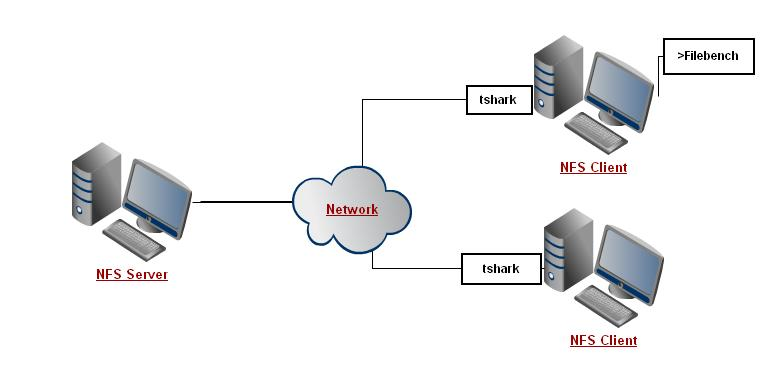
\includegraphics[width=\linewidth]{Arch.jpg}
\caption{Basic architecture of the system}
\label{fig:awesome_image}
\end{figure}

Figure 1 shows the basic architecture of our system. We used VMware Player for setting up NFS server and NFS clients on the virtual machine. filebench workload is generated on the NFS clients after mounting the file system. This generate NFS Call and Reply packets which are collected using tshark running on the client.

\subsection{DataSeries [2]}
We chose the efficient and flexible DataSeries format [2]  - recommended by the Storage Networking Industry Association (SNIA). "DataSeries data model is conceptually very similar to that used by relational databases. Logically, a DataSeries file is composed of an ordered sequence of records, where each record is composed from a set of fields. Each field has a field-type (e.g., integer, string, double, boolean) and a name. A DataSeries record is analogous to a row in a conventional relational database" [2]. 

"A single DataSeries file comprises one or more extents (potentially with different extent-types), a header and extent-type extent at the beginning of the file, and an index extent and trailer at the end of the file. The extent-type extent contains records with a single string-valued field, each of which contains an XML specification that defines the extent-types of all the other extents in the file." [2]

\subsection{Workflow}

\begin{figure}[htb]
\centering
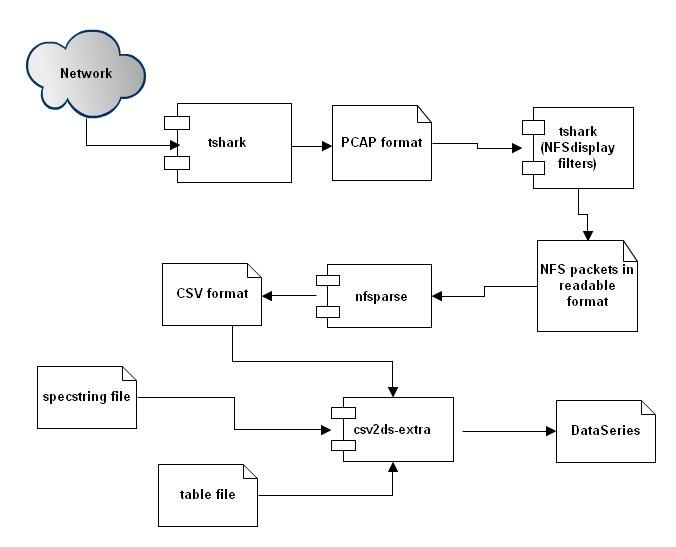
\includegraphics[width=\linewidth]{Flow.jpg}
\caption{Workflow of the system}
\label{fig:awesome_image}
\end{figure}

Figure 2 shows the basic workflow of the system. tshark collects the raw trace information for the workload mentioned above and stores it in the pcap format. The collected trace is again filtered (using tshark nfs display filters) to preserve two important fields in the trace, they are RPC xid and file full paths (optional). RPC xid is a unique id accompanied with each RPC procedure call. NFS v3 supports asynchronous writes and many other operations can be performed asynchronously, so in order to correlate the call and reply of a specific NFS procedure, RPC xid is necessary. This is the reason for preserving RPC xid in the trace information. We have made it mandatory to apply NFS display filter to capture the RPC xid. However, file path snooping is an optional feature which when enabled in tshark will allow our system to capture it in the trace. 

As shown in the Figure 2, the PCAP format is converted into a new readable format containing the fields of our interest. This is fed to "nfsparse" tool which converts it into a csv file. This csv file along with table file of extent types [2] and specification strings [2] file is fed to to the "csv2ds-extra" tool for generating the trace in DataSeries format. Additionally, "nfsstat" (not shown in the figure) will do some basic analysis on the DataSeries file.

\section{Implementation}
We now give the implementation details of our design. We used two virtual machines using VMware Player, one of the virtual machine is configured as NFS server and the other virtual machine is configured as NFS client. Both NFS Server and Client are configured to support NFS V3 protocol.

\subsection{System setup}
We have installed CentOS 6.2 kernel on the virtual machine which is configured as NFS Server and Linux Mint 12 Lisa kernel on the virtual machine which is configured as NFS Client. Using "vmnetcfg" tool which is packaged along with the installation of VMware Player, we have configured both virtual machines to be included in a private "Host-only" network. We have also configured DHCP settings of the "Host-only" network so that it assigns static IP addresses to both server and client. Using the static IP address of the client virtual machine, we have added an entry to the /etc/exports on the server virtual machine for the NFS server to accept and allow NFS requests.

TShark is a network protocol analyzer. It is a terminal oriented version of Wireshark designed for capturing and displaying packets when an interactive user interface isn't necessary or available. It allows us to capture packet data from a live network, or read packets from a previously saved capture file, either printing a decoded form of those packets to the standard output or writing the packets to a file. TShark's native capture file format is libpcap format. We have installed tshark version 1.65 on the NFS Client virtual machine.

Filebench is a file system and storage benchmark that allows to generate a large variety of workloads. We have installed filebench on the client machine to generate workloads and thus capture the ethernet packets which consists of NFS Call and NFS Reply packets using "tshark". Filebench, along with its installation provides with us with a set of predefined scripts which generate the workloads. For our experiments, we have use "fileserver.f" script for generating the workload. This workload is selected because it could generate 11 out of 23 NFS v3 procedures which we thought was reasonable to support in building this prototype system.

\subsection{Capturing and filtering ethernet packets}
tshark is used to capture ethernet packets. These packets contain NFS Call's and Reply's and need to be filtered. In our experiments, we have captured these packets on the NFS Client, but this can be done on the NFS Server side as well. We have used the below command to capture packets using tshark and to store it in PCAP format.\\

\noindent
\# tshark -i \textless interface \textgreater -F libpcap -w \textless output\_file \textgreater\\

\noindent
But these packets need to be filtered for capturing only NFS Call's and Reply's. The above captured PCAP file can be again read using tshark and converted into a readable raw text format using the below command\\

\noindent
\# tshark -r \textless pcap\_file \textgreater -R nfs -t e -z proto, colinfo, rpc.xid, rpc.xid -z proto, colinfo, nfs.full\_name, nfs.full\_name\\

\noindent
This file which is filtered for NFS packets is used in further steps and finally converted into DataSeries format.

\subsection{Defining extent types, table fields, specstrings}
We have defined each NFS Call (and Reply) as a seperate extent-type. The argument for each procedure defines the fields of that particular extent. Some of the fields are obtained only after applying specific NFS display filters on tshark. For such fields, we have set opt\_nullable as "yes" so if they are not present in the trace, the trace can still be converted to DataSeries format.

The extent-type, table fields and spec strings for one such procedure is illustrated below. After converting the raw trace to csv format, the read\_request line is shown as below\\ \\
\noindent
read\_request,5736614403894349824,0xf1667b09,0xda524a8d, 208896, 2872, "192.168.224.129:/home/bigfileset"\\

\noindent
It is not clear what 5736614403894349824, 0xf1667b09, 0xda524a8d, 208896 etc mean.  One needs to define a spec
string that describes the format of the CSV file. The spec string for the same request is defined as \\

\noindent
read\_request(time\_called, xid, file\_handle, offset, length, full\_pathname);\\

\noindent
The table fields describes fields and their types that will constitute target DataSeries file. The table fields for the same request is defined as\\

\noindent 
\textless extent type \textgreater \textless field name \textgreater \textless is nullable? \textgreater \textless field type \textgreater

\noindent
read\_request    time\_called	0      int64\\
read\_request	   xid			0	  variable32\\
read\_request    file\_handle		0       variable32\\
read\_request    offset			0       int64\\
read\_request    length			0       int64\\
read\_request    full\_pathname  1	  variable32\\

Using the table fields, we can generate xml schema. The correspoding xml schema for the extent type is \\

\lstset{breaklines=true}
\lstinputlisting[language=xml]{read_request.xml}

\subsection{nfsparse}
This is a tool developed in C++ which does unit conversion to a CSV file with the fields corresponding to the fields of a target
DataSeries file. It iterates over every line in the raw trace file which is filtered for the NFS packets and generates the CSV file. This CSV file is fed to "csv2ds-extra" tool which converts the CSV to DataSeries format. 

This tool needs a table file which explains the type of the fields in its target DataSeries file. It also need specstrings file which explains the semantics about various fields present in the trace. Below figure illustrates the control-flow of this tool.\\

\begin{figure}[htb]
\centering
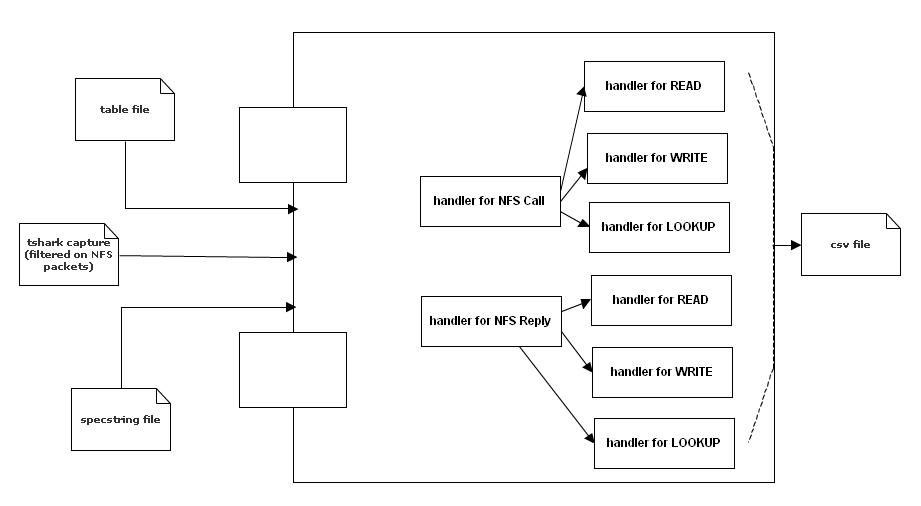
\includegraphics[width=\linewidth]{nfsparse.jpg}
\caption{Functionality of nfsparse}
\label{fig:awesome_image}
\end{figure}

\subsection{nfstrace2ds}
This is a shell script which aggregates all the above operations. The input to this shell script are: 
\begin{itemize}
\item
trace captured by "tshark" in the PCAP format.
\item
table file which explains the semantics of the useful information needed to extract from the trace. 
\item
specstring file which explains the order of the parameters of every procedure in the trace. 
\end{itemize}

\noindent
nfstrace2ds extracts the useful information specified from the trace and generates its equivalent file in DataSeries format. This file could be used to analyze the behavior of the system. It applies several NFS display filters on the PCAP trace file and extracts the NFS Call's and Reply's. We have used "-R nfs -t e -z proto,colinfo,rpc.xid,rpc.xid -z proto,colinfo,nfs.full\_name,nfs.full\_name" tshark options for filtering the NFS packets. "tshark" allows file path to full name snooping if it learns the file names before the file system is mounted by the client. The option "-z proto,colinfo,nfs.full\_name,nfs.full\_name" is made optional but rpc.xid is needed for analyzing the traces where we need to correlate between NFS Call and NFS Reply. The result of this filtered NFS trace is then stored in a temporary file which is used to invoke "nfsparse" which generates csv file for the given trace. This along with the table file and specstring file is fed to "csv2ds-extra" tool which is a part of DataSeries to convert the trace file to its corresponding DataSeries format.

\subsection{nfsstat}
This is a analyzer module which processes the trace in the DataSeries format. It uses the DataSeries API to perform some basic analysis on the traces. It tabulates the procedure counts (READ, WRITE, GETATTR, LOOKUP etc) for the workload which generated the traces. It also captures I/O sizes of the READ and WRITE procedures over the trace. This data can be used for analyzing mean I/O size for READ and WRITE procedures and also determining the behaviour of the system such as read-heavy or write-heavy etc.
\section{Analysis and Evaluation}
As a part of our system, we have developed a small analyzer module which performs some basic analysis on the trace which we have converted into DataSeries format. We have used DataSeries RowAnalysis API for reading the DataSeries file. "nfsstat" is the module which reads the trace and displays the statistics about NFS V3 procedures. The results of our converter and analyzer are evaluated with "dsstatgroupby" tool which is a part of DataSeries installation tools.

\noindent
In our experiments, we ran "fileserver" workload for 5 seconds and collected the trace using tshark in PCAP format using the command \\

\noindent
tshark -i \textless interface \textgreater -F libpcap -w \textless output\_file \textgreater\\

\noindent
On the captured PCAP format,we have applied NFS display filters to extract desirable properties using the following command\\

\noindent
tshark -r \textless pcap\_file \textgreater -R nfs -t e -z proto, colinfo, rpc.xid, rpc.xid -z proto, colinfo, nfs.full\_name, nfs.full\_name \\

\noindent
This is fed to "nfsparse" followed by "csv2ds-extra" to convert it into DataSeries format. The DataSeries file is fed to "nfsstat". "nfsstat" iterates through each and every row in the DataSeries file. fileserver workload was able to generate 11 different types of NFS V3 procedures. During 5 seconds of the workload, we analyzed number of times each procedure is requested by the NFS Client. Figure 4 displays the number of times specific NFS V3 procedure is requested.\\

\noindent
\begin{figure}[htb]
\centering
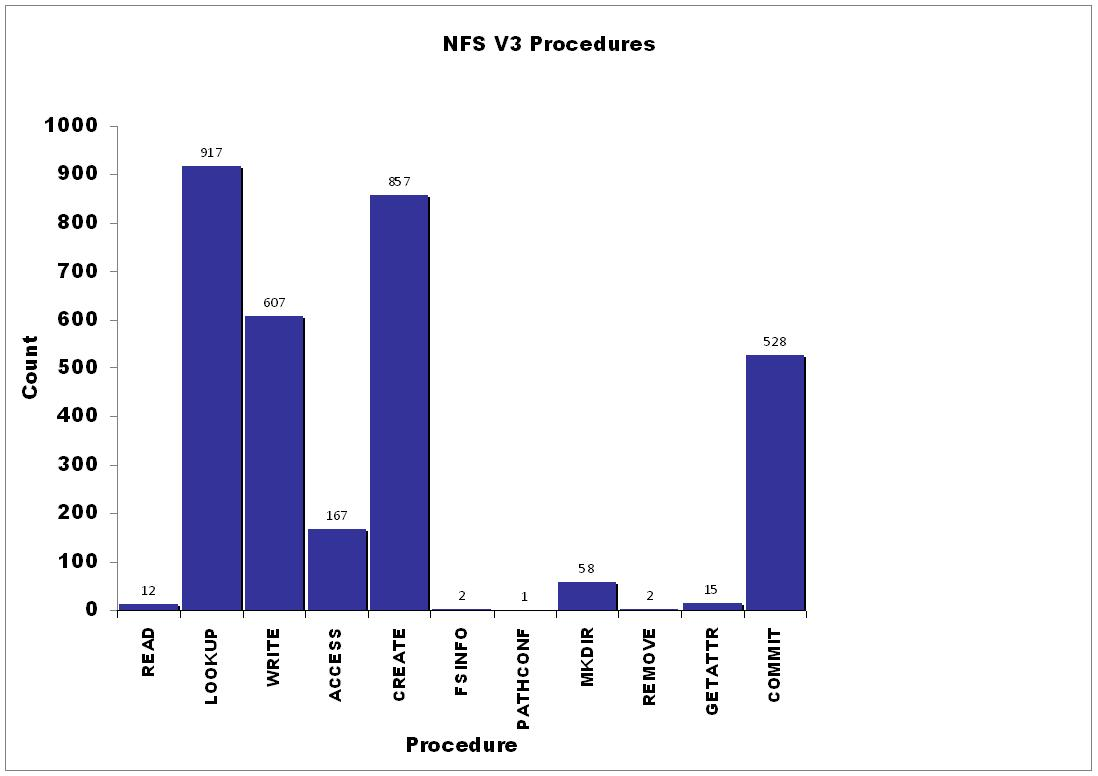
\includegraphics[width=\linewidth]{procedure_count.jpg}
\caption{NFS Procedure vs Count}
\label{fig:awesome_image}
\end{figure}

The table below displays the NFS V3 procedure counts observer during our experiment.

\noindent
\begin{center}
    \begin{tabular}{|c|c|}
        \hline
        PROCEDURE & COUNT  \\ \hline
        READ      & 12       \\ \hline
        WRITE      & 607       \\ \hline
        LOOKUP      & 917       \\ \hline
        ACCESS      & 167       \\ \hline
        CREATE     & 857       \\ \hline
        FSINFO      & 2       \\ \hline
        PATHCONF      & 1       \\ \hline
        MKDIR      & 58       \\ \hline
        REMOVE      & 2       \\ \hline
        COMMIT      & 528       \\ \hline
        GETATTR     & 15   \\
        \hline
    \end{tabular}
\end{center}

$\newline$

"nfsstat" also calculates the mean, standard deviation of I/O sizes for the READ and WRITE procedures. The results of the analyzer are evaluated with DataSeries tools. The table below displays the results of "nfsstat" for the fileserver workload.\\

\noindent
\begin{center}
    \begin{tabular}{|c|c|c|c|}
        \hline
        PROCEDURE & COUNT & MEAN    & STD DEVIATION \\ \hline
        READ      & 12    & 36021.4 & 29949.7       \\ \hline
        WRITE     & 607   & 44562.3 & 22332.8       \\
        \hline
    \end{tabular}
\end{center}

$\newline$

We have also analyzed the I/O sizes of the READ and WRITE procedures. The fileserver worload is observed to have more WRITE procedures when compared to the READ procedures. Figure 5 and 6 plots the graphs between I/O size and its corresponding READ and WRITE procedures. 
\noindent
\begin{figure}[htb]
\centering
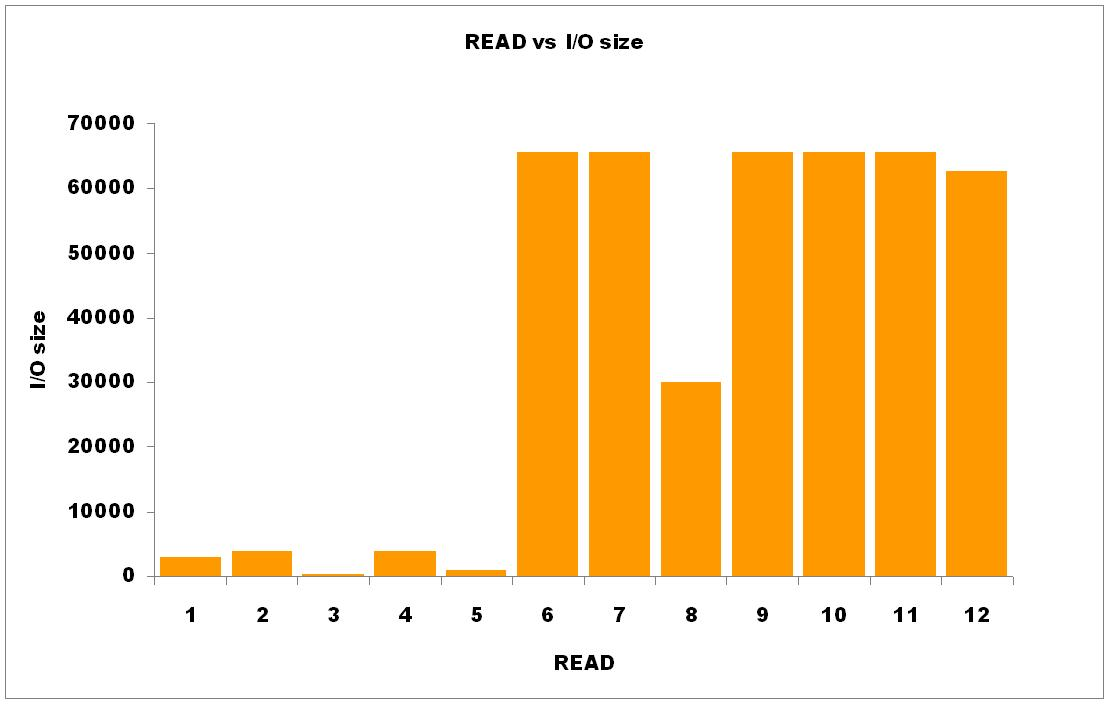
\includegraphics[width=\linewidth]{read_io.jpg}
\caption{NFS READ Procedure vs I/O size}
\label{fig:awesome_image}
\end{figure}


\noindent
\begin{figure}[htb]
\centering
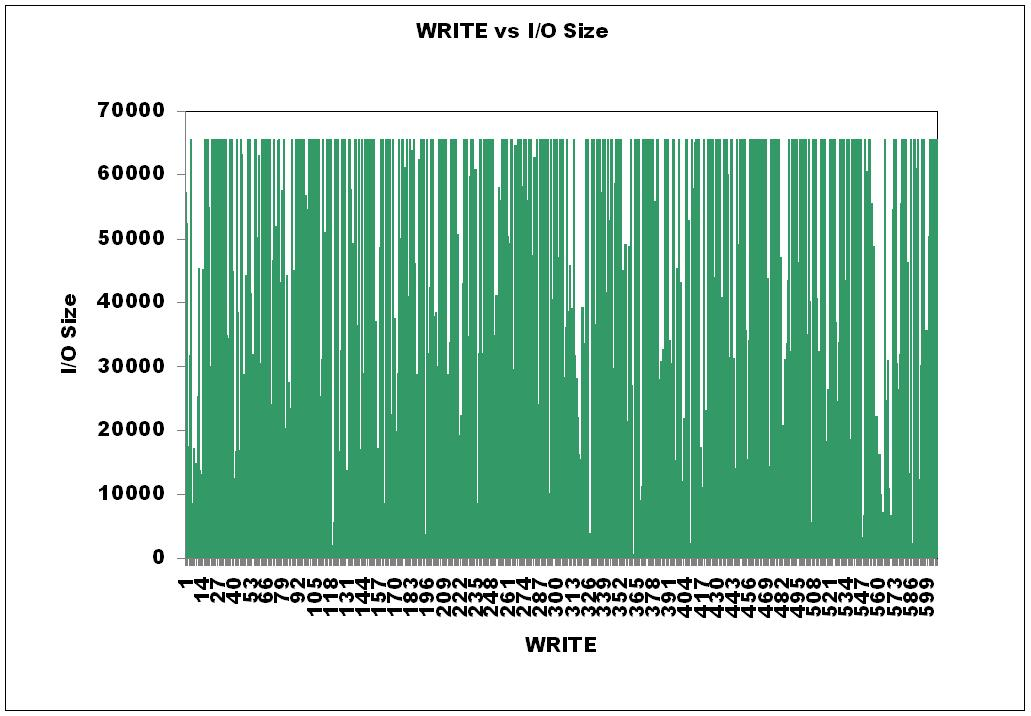
\includegraphics[width=\linewidth]{write_io.jpg}
\caption{NFS WRITE Procedure vs I/O size}
\label{fig:awesome_image}
\end{figure}
\noindent

\section{Conclusion and Future Work}
NFS traces provide a wealth of information about an NFS workload. Our system simplifies extracting this information
and performs some useful analysis. We have created a system that currently supports only 11 NFS V3 procedures i.e. CREATE, READ, WRITE, LOOKUP, GETATTR, ACCESS, REMOVE, MKDIR, FSINFO, PATHCONF, COMMIT. If the trace captured contains other procedures, our system will ignore the packets and continue further. In future we plan to extend the system to support all other procedures. We have also built a small analyzer module "nfsstat" which does some very basic analysis on the DataSeries file as described in the above sections. We can extend the functionality of this module to perform some advance statistical analysis which would be helpful in understanding the system behaviour.

Also, we can integrate this system with T2M [7] to generate workload models from the traces for certain benchmark tools for understanding complex distributions in real-world traces.


% conference papers do not normally have an appendix


% use section* for acknowledgement
\section*{Acknowledgment}

The authors would like to thank Professor Erez Zadok and Vasily Tarasov for their valuable help and guidance thoughout the project.

% trigger a \newpage just before the given reference
% number - used to balance the columns on the last page
% adjust value as needed - may need to be readjusted if
% the document is modified later
%\IEEEtriggeratref{8}
% The "triggered" command can be changed if desired:
%\IEEEtriggercmd{\enlargethispage{-5in}}

% references section

% can use a bibliography generated by BibTeX as a .bbl file
% BibTeX documentation can be easily obtained at:
% http://www.ctan.org/tex-archive/biblio/bibtex/contrib/doc/
% The IEEEtran BibTeX style support page is at:
% http://www.michaelshell.org/tex/ieeetran/bibtex/
%\bibliographystyle{IEEEtran}
% argument is your BibTeX string definitions and bibliography database(s)
%\bibliography{IEEEabrv,../bib/paper}
%
% <OR> manually copy in the resultant .bbl file
% set second argument of \begin to the number of references
% (used to reserve space for the reference number labels box)
\begin{thebibliography}{1}

\bibitem{IEEEhowto:kopka}
Extracting Flexible, Replayable Models from Large Block Traces - V.
Tarasov, S. Kumar, J. Ma, D. Hildebrand, A. Povzner, G. Kuenning, and
E. Zadok Stony Brook University, Harvey Mudd College, and IBM Almaden
Research
\bibitem{IEEEhowto:kopka}
DataSeries: An efficient, flexible data format for structured serial data
- DataSeries Technical Documentation
\bibitem{IEEEhowto:kopka}
VFS Interceptor: Dynamically Tracing File System Operations in real
environments - Yang Wang, Jiwu Shu, Wei Xue , Mao Xue
\bibitem{IEEEhowto:kopka}
New NFS Tracing Tools and Techniques for System Analysis - Daniel
Ellard and Margo Seltzer
\bibitem{IEEEhowto:kopka}
Capture, conversion, and analysis of an intense NFS workload - Eric
Anderson, HP Labs
\bibitem{IEEEhowto:kopka}
RFC 1813 - NFS Version 3 Protocol Specification
\bibitem{IEEEhowto:kopka}
T2M: Converting I/O Traces to Workload Models - Vasily Tarasov (student, presenter), Koundinya Santhosh Kumar (student)
and Erez Zadok (Stony Brook University)
Geoff Kuenning (Harvey Mudd College)
\end{thebibliography}



% that's all folks
\end{document}


